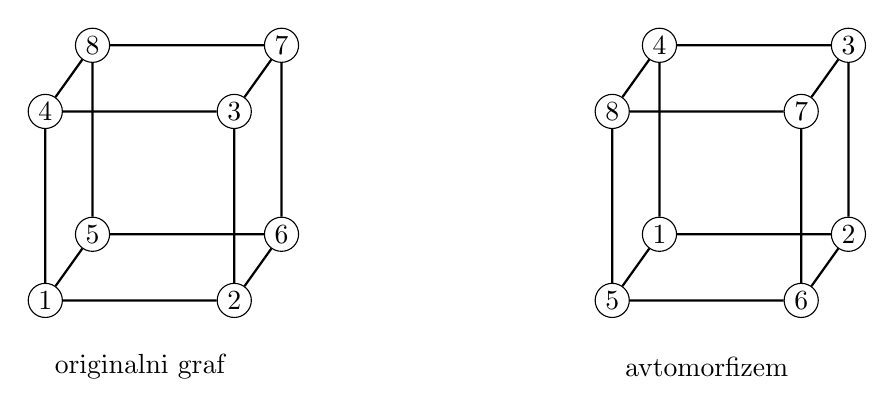
\begin{tikzpicture}[scale=1.2,
    v/.style={circle, draw, fill=white, inner sep=1.5pt},
    e/.style={thick}
]

    % Originalna kocka
    \begin{scope}[shift={(-3,0)}]

    % vertices
    \node[v] (a1) at (0,0) {$1$};
    \node[v] (a2) at (2,0) {$2$};
    \node[v] (a3) at (2,2) {$3$};
    \node[v] (a4) at (0,2) {$4$};

    \node[v] (b1) at (0.5,0.7) {$5$};
    \node[v] (b2) at (2.5,0.7) {$6$};
    \node[v] (b3) at (2.5,2.7) {$7$};
    \node[v] (b4) at (0.5,2.7) {$8$};

    % bottom square
    \draw[e] (a1)--(a2)--(a3)--(a4)--(a1);

    % top square
    \draw[e] (b1)--(b2)--(b3)--(b4)--(b1);

    % vertical edges
    \draw[e] (a1)--(b1);
    \draw[e] (a2)--(b2);
    \draw[e] (a3)--(b3);
    \draw[e] (a4)--(b4);

    \node at (1, -0.7) {originalni graf};

    \end{scope}


    % Avtomorfizem
    \begin{scope}[shift={(3,0)}]

    % vertices (permuta oznak)
    \node[v] (c1) at (0,0) {$5$};
    \node[v] (c2) at (2,0) {$6$};
    \node[v] (c3) at (2,2) {$7$};
    \node[v] (c4) at (0,2) {$8$};

    \node[v] (d1) at (0.5,0.7) {$1$};
    \node[v] (d2) at (2.5,0.7) {$2$};
    \node[v] (d3) at (2.5,2.7) {$3$};
    \node[v] (d4) at (0.5,2.7) {$4$};

    % bottom square
    \draw[e] (c1)--(c2)--(c3)--(c4)--(c1);

    % top square
    \draw[e] (d1)--(d2)--(d3)--(d4)--(d1);

    % vertical edges
    \draw[e] (c1)--(d1);
    \draw[e] (c2)--(d2);
    \draw[e] (c3)--(d3);
    \draw[e] (c4)--(d4);

    \node at (1,-0.7) {avtomorfizem};

    \end{scope}

\end{tikzpicture}